% V166 owned review; user-supplied mcmthesis format, shared class unchanged.
\documentclass{mcmthesis}
\mcmsetup{CTeX=false,tcn=PENDING,problem=A,sheet=true,titleinsheet=true,
keywordsinsheet=true,titlepage=false,abstract=true}
\usepackage{palatino,microtype,ragged2e,placeins,url,xurl}
\setlength{\headheight}{16pt}\urlstyle{same}\emergencystretch=3em\hyphenpenalty=500
\AtBeginDocument{\setlength{\parindent}{0pt}\setlength{\parskip}{0.5\baselineskip}}
\setlength{\tabcolsep}{5pt}
\widowpenalty=10000\clubpenalty=10000
\setcounter{tocdepth}{2}
\makeatletter
\renewcommand\tableofcontents{%
\centerline{\rmfamily\Large\bfseries\contentsname%
\@mkboth{\MakeUppercase\contentsname}{\MakeUppercase\contentsname}}%
\vskip 3ex\@starttoc{toc}}
\renewcommand{\l@section}{\def\@pnumwidth{2.3em}\def\@tocrmarg{2.3em}%
\bfseries\@dottedtocline{1}{1.5em}{2.3em}}
\renewcommand{\l@subsection}{\normalfont\@dottedtocline{2}{3.0em}{3.2em}}
\renewcommand{\@dotsep}{1}
\makeatother
\title{Choosing a City for High-School Life with Incomplete Evidence}
\author{}\date{}
\hypersetup{pdftitle={Choosing a City for High-School Life with Incomplete Evidence},pdfauthor={}}
\graphicspath{{./}{drafts/}}
% V154 data and controlled extensions; V148 historical cases retained.
\newcommand{\EquityCase}{A separate Shanghai school-resource case uses 16 districts, 235,542 regular senior-secondary pupils and 23,999 full-time teachers in the 2025 school year. The pooled utility is 0.604481; the student-weighted mean of district utilities is 0.603267. Ordering districts by resource utility and averaging the bottom 20\% of pupil mass, with fractional inclusion of the boundary district, gives 0.580954, 0.022313 below the weighted mean. These are district-homogeneous school-location resource scenarios, not observed individual teacher exposure or resident accessibility \cite{shanghai}.  }
\newcommand{\AgeCase}{A historical Istanbul household survey offers current-high-school groups aged 14--15 and 16--18. Their travel-utility marginal bounds overlap: $[0.35961,0.55711]$ and $[0.29347,0.59346]$, respectively. They include unknown durations and optional members; shared unknown-age mass means their extrema need not be jointly attainable. They describe 2012 broad groups, not exact ages fourteen and eighteen today. Singapore's MOE table records 38,555 students aged fourteen and only 165 aged eighteen at the start of 2020 still in secondary schooling; the latter is not an all-eighteen-year-old resident denominator. These counts cannot be joined to census school-stage travel bins without a matching population/reference-day table \cite{istanbul,sgage}.  }
\newcommand{\CountryInterpretation}{Phoenix has higher retained affordability utilities than New York. Mumbai has the higher PM$_{2.5}$ utility, while Delhi has higher living-cost, housing, school-resource and broadband utilities in the retained evidence. The cases inherit the historical study's geographic and educational scope; their score pairs overlap, so neither case identifies a necessary overall winner.  }
\newcommand{\CaseReferences}{\bibitem{shanghai} Shanghai Municipal Education Commission. Regular secondary-school pupil and teacher tables, school year 2025. \url{https://edu.sh.gov.cn/xxgk2_zhzw_tjsj_01/20260610/890926a33cbf443d9abf07c6f65b7734.html}. \bibitem{istanbul} Istanbul Metropolitan Municipality. 2012 household transport survey, official data-portal response resource \texttt{a75118db-28c9-4fdf-b367-d5933b7bb810}; questionnaire, report and nonidentifying aggregate audit archived. \bibitem{sgage} Singapore Ministry of Education. Secondary enrolment by level and age, 2020. \url{https://data.gov.sg/datasets/d_cc84fc751ef5106d9e26cfdbf61776c8/view}.  }
\newcommand{\CurrentMeanWidth}{16.06144}
\newcommand{\TotalWidthReduction}{14.62}
\newcommand{\LatestEvidenceChange}{The Milan metro subset narrows the preceding fixed-weight mean from 16.08933 to 16.06144. The 104 retained station/hub entities raise one utility lower bound while all static decision ranks remain unchanged. This is an information update using a dated inventory, not an observed improvement over time. }
\newcommand{\RevisionRankChanges}{13}
\newcommand{\SummaryWeightMC}{In 10,000 baseline weight perturbations at Dirichlet concentration 100, Zurich is recommended in 43.33\% of draws, compared with 27.92\% for Oslo and 28.23\% for Singapore. }
\newcommand{\MethodComparison}{TOPSIS selects Zurich at the midpoint, whereas VIKOR selects Dublin; Kendall's $\tau_b=0.500$. Dublin satisfies VIKOR's advantage and stability conditions. Under equal weights, $\tau_b=0.650$; Oslo has the lowest VIKOR index but fails those acceptance conditions, so it is not an accepted unique compromise solution. }
\newcommand{\FutureDeterministic}{All three uniform-change scenarios retain Zurich as the conservative recommendation and all sixteen cities as possible champions under both weight references, including the Singapore-proxy withdrawal arm. Balanced improvement changes the fixed-weight second and third decisions from Singapore--Oslo to Oslo--Singapore.  }
\newcommand{\FutureThresholds}{Oslo reaches the tie at approximately 5.685\% reduction, Singapore at 10.309\%, and Stockholm at 28.875\%. Zurich already minimizes regret at baseline. A slightly greater reduction produces a strict recommendation switch in these calculations. }
\newcommand{\FutureMonteCarlo}{Specifically, $C\sim U[0,1]$ is shared across cities and $I_i\sim U[0,1]$ varies by city, independently; $\delta_i=0.05C+0.05I_i$. The relevant raw multipliers are $1+\delta_i$ or $1-\delta_i$, and affected criteria within a city share that multiplier. With 10,000 draws per scenario, Zurich's fixed-weight recommendation frequencies are 100.00\%, 96.85\%, 97.72\% for resource expansion, living pressure and balanced improvement respectively. }
\newcommand{\ProxyWithdrawalMC}{Repeating the same shocks after withdrawing Singapore's historical stage-travel proxy gives 100.00\%, 99.19\%, 97.72\% respectively. These paired calculations isolate dependence on that proxy while retaining the chosen shock distribution. }
\newcommand{\PreferenceResults}{Education priority changes the conservative recommendation from Zurich to Oslo, with decision-rank $\tau_b=0.733$ relative to baseline. Independent-living priority retains Zurich and gives $\tau_b=0.883$. All sixteen cities remain possible champions in each profile. }
\newcommand{\PreferenceEvidenceChange}{At concentration 100 around baseline weights, Milan's mean decision rank changes from 13.3073 to 12.9648 after its inventory supplement. The fixed education-priority recommendation remains Oslo; these are changes in the declared evidence bounds and weight distribution. }
\newcommand{\EvidenceThresholdCheck}{Berlin's hypothetical combined-cost tie threshold is 38.084\% after the Milan inventory update. Scenario definitions and weights are unchanged. }
\newcommand{\MonteCarloInterpretation}{At concentration 100, Oslo has a better mean decision rank (2.1092) than Zurich (2.2620), although Zurich has the greater recommendation frequency and is the fixed-weight minimax choice. These summaries answer different questions about the chosen weight distribution. }

\begin{document}
\begin{abstract}
A city recommendation becomes more useful when its evidence and priorities can
be examined together. We compare sixteen cities using ten indicators of safety,
environment, household costs, education and everyday resources. Zurich is the
conservative recommendation under the retained team inputs and baseline or equal weights. All sixteen
cities remain possible champions within the retained evidence bounds.

The evaluation combines fixed-anchor TOPSIS with a maximum-regret decision.
Benefit and cost utilities share fixed reference scales, allowing controlled
comparisons across data, preference and development scenarios. Missing values
remain intervals. We select the city with the smallest worst-case shortfall from
a better-scoring competitor over the declared rectangular uncertainty set.

Official municipal records, school statistics and operator inventories supplement
twenty-two previously missing entries while preserving the team's original values.
The average score-interval width falls from 18.81077 to \CurrentMeanWidth{}, a \TotalWidthReduction\%
reduction. Actual reference years and source
populations remain explicit.

A controlled formulation revision retains the 48 uncertain entries rather
than collapsing each to a midpoint. Although Zurich remains the recommendation, \RevisionRankChanges{}
fixed-weight decision ranks change. Separate interior completions let each of the sixteen cities rank first.
Withholding Zurich's unverified homicide-rate point alone selects Singapore
under baseline weights and Oslo under equal weights, exposing dependence on
accepted source information.

Preferences and development conditions answer different decision questions.
Doubling the relative emphasis on education changes the conservative choice to
Oslo. \SummaryWeightMC{} These are conditional simulation frequencies.
Three uniform ten-per-cent development scenarios retain Zurich; separate
city-specific shocks reveal conditional recommendation changes without claiming
an empirical forecast.

Separate country, district and age-group cases examine what citywide totals
leave unresolved. They distinguish facility supply from student access and
observed broad age groups from unsupported age-specific preferences. The result
is a practical starting choice with explicit alternatives and clear priorities
for additional evidence.
\begin{keywords}
high-school opportunities; TOPSIS; interval evidence;
maximum regret; preference sensitivity.
\end{keywords}
\end{abstract}
\maketitle
\clearpage
\tableofcontents
\clearpage
\section{Introduction and decision scope}
\subsection{What makes a city suitable for high-school life?}
A useful comparison connects a student's school day with the opportunities and
constraints around it. Safety and air quality affect the daily setting; teaching
resources and nearby higher education describe educational supply; housing,
living costs, transport, travel, broadband and swimming facilities describe
household pressures and everyday resources. Our operational definition of
``best'' is the conservative choice under these ten criteria, declared weights
and retained evidence ranges. It provides a starting recommendation for the
compared cities, rather than a claim about every student's experience.

The study uses the sixteen cities in the frozen team matrix: Amsterdam, Berlin,
Dublin, Helsinki, London, Madrid, Milan, Oslo, Paris, Prague, Singapore,
Stockholm, Tokyo, Vienna, Warsaw and Zurich. This is an inherited comparison
set across sixteen countries, not a representative sample of all world cities.
It exceeds the problem's minimum of ten cities and spans different resource
and cost settings. The findings concern this set; a broader claim would require
an explicit sampling design and additional comparable observations.

\subsection{Criterion selection and contribution}
The ten indicators preserve the agreed team framework and balance education
with the conditions that make resources usable in daily life. Their directions
and anchors appear in Table~\ref{tab:indicators}. Counts and city averages serve
as scoped supply or setting measures. They do not directly measure friendships,
student wellbeing, school quality, language fit, discrimination, cultural
participation or individual access. Those outcomes are relevant to a family's
choice; comparable student-level observations are needed to integrate them
without inventing measurements or double-counting existing proxies.

Our central contribution is a city decision that retains incomplete evidence.
We improve source precision, compare a point-completion benchmark with an
interval revision, and examine preferences and future conditions without
changing the primary indicator set. TOPSIS provides one main quality score;
AHP structures stated priorities, Monte Carlo measures specified perturbations,
and VIKOR supplies a focused method comparison. The extensions test the
recommendation rather than vote among an expanding set of ranking models.

AI assistance supported research retrieval, calculations, code and prose
preparation, including Exa source retrieval and extraction \cite{openai,exa}.
The appended use report records the known assistance
and the outstanding documentation required before submission.

\section{Assumptions and their role}
\begin{enumerate}
\item \textbf{Comparability follows the retained scope.} Original values and
population denominators remain fixed. Each supplement keeps its provider,
year, city boundary and educational population. Mixed-year densities are
conditional comparisons; they do not create a same-year census.
\item \textbf{Utilities are monotone on fixed scales.} More resources and less
cost or burden improve their respective utilities. Declared anchors set the
scale; they are neither estimated preferences nor empirical optimum values.
\item \textbf{The score permits compensation.} Weighted distances combine
criteria in a common utility space. The model therefore allows stronger results
on some criteria to offset weaker results on others. A family requiring a hard
safety or eligibility threshold should apply it separately before choosing.
\item \textbf{The evidence set is rectangular.} Uncertain utilities vary
independently within retained intervals. This conservative closure omits unknown
cross-criterion and cross-city restrictions. Its possible champions and regret
bounds are conditional on this set; they are not population probabilities.
\item \textbf{Extensions hold the comparison basis fixed.} Scenario changes
retain population denominators, anchors and the indicated weight rule. They
are conditional experiments with no fitted future date or representative
age-specific preference distribution.
\end{enumerate}

\section{Notation}
\begin{tabular}{p{.18\linewidth}p{.75\linewidth}}
\toprule Symbol & Meaning\\\midrule
$M,N$ & Sixteen cities and ten indicators\\
$w_j,a_j$ & Normalized criterion weight and fixed utility anchor\\
$u_{ij}$ & Utility of indicator $j$ for city $i$, on $[0,1]$\\
$\ell_{ij},h_{ij}$ & Retained lower and upper utility bounds\\
$L_i,U_i$ & Lower and upper TOPSIS score, on $[0,100]$\\
$R_i,\mathcal C$ & Maximum regret and set of possible champions\\
$\kappa$ & Concentration of a declared Dirichlet weight distribution\\
$r$ & Raw-value multiplier in a development scenario\\\bottomrule
\end{tabular}

% Owned V123 contribution rebased to V154 evidence and established controlled extensions.
\section{Data collection and comparability}
\subsection{A traceable city--indicator matrix}
We compare $M=16$ cities on $N=10$ indicators covering safety, environment,
household costs, education and everyday resources. The initial matrix is the
team-supplied city table \cite{teamtable}. We retain its existing values, populations, reference
years and source flags as the agreed input, then supplement only empty cells.
Some supplied values lack original source URLs, so their provenance remains
the team table; official supplements do not retrospectively validate every
supplied measurement. Table~\ref{tab:indicators} states what each variable measures.

\begin{table}[htbp]\centering
\caption{Retained indicators, units and reference anchors. Supplied values are retained; supplements have explicit source scope.}\label{tab:indicators}
\begin{tabular}{p{.22\linewidth}p{.56\linewidth}r}
\toprule Indicator & Measurement and interpretation & Anchor\\\midrule
Homicide & Deaths per 100,000; cost; supplied city proxy & 2 \\
PM$_{2.5}$ & $\mu$g/m$^3$; cost; supplied concentration proxy & 15 \\
Living costs & Supplied living-cost index; cost & 100 \\
Housing & Supplied price-to-income ratio; cost & 10 \\
School resources & Pupils per teacher or explicitly scoped FTE; cost & 15 \\
Higher education & Institutions per 100,000; benefit; supply proxy & 1 \\
Transport stops & Unique stops per 100,000; benefit; partial inventories & 50 \\
Travel & Duration in minutes; $\exp(-t/30)$; commute or stage proxy & 30 min \\
Broadband & Supplied Mbps; benefit; city/general-use proxy & 100 \\
Swimming pools & Venues per 100,000; benefit; supply proxy & 1 \\
\bottomrule
\end{tabular}
\end{table}


The nominal reference year is 2025, but the evidence is mixed-vintage. Every
supplement retains its actual year rather than being relabelled as 2025.
Population denominators remain those of the supplied table. Thus a 2026 facility
snapshot divided by a supplied 2025 population is a conditional density, not an
observed same-year census. We do not infer that facilities are unchanged merely
because they may change slowly. Historical inventory assumptions are evaluated
through withdrawal scenarios.

We use official statistical tables, operator inventories and municipal geodata
to fill missing fields. For each admitted supplement, the archive records the
provider, URL, year, geographic and population scope, units, extraction rule and
file hash. Original PDFs and API responses are retained separately from derived
tables. Search summaries locate evidence; numerical admission requires the
underlying record or an explicitly identified provider capture. Values are
converted to compatible units before utility calculation: for example, the
supplied higher-education density per million is divided by ten to obtain the
per-100,000 scale. Mode share is not converted into physical stop density.

\subsection{Collection problems and their resolution}
\textbf{A station is not a platform, and a network is not a city.}
Oslo's municipal GIS represents platforms. Selecting records within the city
boundary and consolidating names gives 89 metro stations from 186 platforms.
Zurich's official 2025 VBZ report separately lists 446 stops on city territory
and 235 in the surrounding area; only 446 enter the city inventory
\cite{oslo,vbz}. A November 2026 snapshot of Helsinki's operator similarly
distinguishes 19 metro stations in Helsinki from 11 in Espoo \cite{helsinki}.
These are mode or operator subsets, so they supply
lower bounds rather than complete all-operator totals. For a verified facility
count $c$ and fixed population $P$, density is $d=10^5c/P$; utility is bounded by
$[d/(a+d),1]$.

Madrid's metro register contains 293 records. Of these, 242 carry code 28079 for the city, independently confirmed by INE. Omitting two unnamed records without lines and consolidating 240 named records by the provider's network-station identifier yields 191 city complexes. Linked multi-name complexes are conservatively counted once; 51 outside-city records are excluded \cite{madridmetro,inecodes}. This is a 29 May 2026 registered inventory with the supplied 2025 population, not a real-time operating count.

\textbf{A transport register can include non-passenger objects.}
Vienna's versioned operator files group stopping positions into DIVA station
areas. A broad route-pattern extraction yields 1,695 named city areas, but it
includes depot objects whose passenger-stop status is unproved. We reject that
count and retain 99 metro areas matched individually to the city's separate
existing-station layer and administrative polygon \cite{viennaogd,viennagis}.
Explicit spelling aliases are checked against both names and coordinates;
110 line appearances are not counted as 110 complexes. The 8 November 2026
export uses the unchanged supplied 2025 population. Its inventory membership
does not guarantee a departure or unrestricted access at a particular time.

Prague's current city-classified PID list supplies 57 named metro complexes
with route timetables \cite{pidmetro}. M\r{u}stek, Muzeum and Florenc each
count once despite two serving lines. The 2025 DPP report has 61 line
appearances and 58 distinct complexes; the current subset omits Flora,
whose 2026 closure is corroborated by the operator \cite{dpp2025,floraclose}.
Florenc's partial accessibility restriction does not close the whole complex.
Both supplements retain upper utility 1 for uncounted facilities.

Berlin's nine official U-Bahn route profiles contain 131 station appearances
in tariff zone A, defined by BVG as the Berlin inner city through the S-Bahn
ring. Native station identifiers consolidate these to 100 complexes; normalized
names are bijective with identifiers and cross-line transfers corroborate
repeated appearances \cite{bvg}. We retain this inner-city subset and leave
outer stations and other modes uncounted. The November 2026 published inventory
uses the supplied 2025 population; it measures registered resources rather
than real-time service or a student's individual access.

Milan's municipal station layer supplies 130 records, of which 109 have both the Milano municipality name and code 015146. Consolidating the five line-specific interchange pairs identified on the operator map leaves 104 station/hub entities; 21 records without matching geography are omitted. The station layer is distinguished from its entrance layer, and proximity alone does not merge adjacent stations. Its stated inventory date is 16 October 2024; with the unchanged supplied 2025 population, it provides a historical lower-bound proxy rather than an exact 2025 count or current-service census \cite{milanmetro}.

London's TfL inventory contains 1,751 mixed objects, including platforms and entrances. Of 272 station-level records, 62 have the exact fare-zone value 1. Omitting two records conservatively and consolidating Paddington's shared native hub leaves 59 station/hub entities; all retained representative coordinates lie within the ONS December 2025 London-region boundary \cite{tflinventory,onslondon}. This November 2026 inventory uses the unchanged supplied 2025 population. It raises the resource lower bound while leaving other zones and operators uncounted; it does not establish individual access.

\textbf{A list of venues can contain closed facilities.}
Stockholm's current municipal swimming directory lists fourteen named venues,
one of which is explicitly closed for renovation. The thirteen retained venues
agree with the current overview; the temporary year-round replacement is
counted once \cite{stockpool}. We count venues, not individual basins. This
municipal subset gives a supply lower bound and leaves other providers unknown.
Its access date is November 2026; a page-footer date is not used to reconstruct
a 2025 inventory. Paris's 244 intra-muros metro stations come from a March 2022
atlas using RATP 2021 and Apur 2022 sources, not a 2025 observation
\cite{apur}. A separate withdrawal restores this historical supplement to unknown.

Tokyo's retained municipal subset consists of five indoor swimming venues at different Nerima addresses, verified against original city pages with 25-metre specifications. Heiwadai's current closure with no reopening date excludes it; Miharadai's announced February--May 2027 closure is distinguished from current stock \cite{nerimapool,nerimaclose}. Other wards/providers remain uncounted. The count measures venues, not lanes, basins or simultaneous opening.

\textbf{Pupils and teachers must refer to the same schools and stage.}
Prague's 2024/25 tables report 80,073 secondary-school pupils and 6,877.1
teacher full-time equivalents (FTE), including lower-gymnasium years.
Subtracting the matching 8,748 pupils and 737.8 FTE yields 71,325 pupils and
a rounding envelope of $[6139.2,6139.4]$ FTE \cite{prague}. The Prague
measure includes all study modes, including adult and non-daytime cohorts.
Stockholm's
published city-school ratio covers upper-secondary years 1--3 and all provider
ownership types, measured on 15 October \cite{kolada}. Its API value
16.42091405 is conservatively represented by $[16.35,16.45]$, an intentional
precision convention rather than a claimed measurement-error confidence interval.
Henri-IV (Paris, UAI 0750654D) reports 794 lyc\'ee pupils and 153.65
institution FTE for 2025, without an upper-stage allocation or complete
city-provider coverage \cite{deppmatch}. A 2026 post-baccalaureate flag cannot
recover its 2025 workloads \cite{deppdirectory}.
Dublin's school-roll payroll FTE are unpublished \cite{irelandfte}.
Its November 2025 City Of Dublin ETB post-primary vocational subgroup reports
411.8 payroll FTE against 376.1 allocated posts \cite{irelandpayroll}:
allocation is not a payroll ceiling, and this subgroup does not identify the
city's PTR. Finland's national FTE uses salary and private-provider data for
estimation, alongside register sources. Without a verified one-sided error
envelope, we do not use that estimate as a guaranteed Helsinki teacher upper
bound \cite{finlandfte}. All three city PTRs remain unknown.

\textbf{Rates require matching units and denominators.}
CBS's 2023 release gives ten provisional homicide victims in Amsterdam in 2022;
its regional workbook instead totals 68 over 2018--2022. Neither matches the
supplied numerator 340 \cite{cbshomicide2022}. Zurich's PKS report lists one
completed offence in 2024 and two in 2025. Its glossary counts criminal acts
independently of victims, and the submitted rate of 0.14 still lacks a verified
denominator \cite{zhpks2025}. We retain both original entries and test their
information contribution in Section~\ref{sec:sourcepolicy}, without constructing
replacement rates across incompatible units.

\textbf{Unavailable records and unobserved travellers are retained honestly.}
An initial Singapore census PDF endpoint returned 404; the official Parliament
mirror and official data API supplied the report and matching table
\cite{singapore}. Duration bins are converted using utility at their endpoints,
without bin midpoints or an artificial maximum duration for the open tail.
The stage-specific total enrolment estimates exceed the travel-table estimates
by estimated uncovered student totals of 1,811 for secondary, 989 for
post-secondary non-tertiary and 1,635 for polytechnic. These are weighted
survey estimates rather than complete headcounts. The uncovered mass retains
utility $[0,1]$; unknown stage proportions are
handled by the interval convex hull. The resulting $[0.21048,0.61884]$ is a
2020 school-stage proxy, not an identified 2025 interval for ages 14--18.
When Dublin raw stop downloads returned 403, no count was inferred from the
catalogue. A later official map supported a separately documented subset of
19 existing city-centre tram stops \cite{dublin}. Warsaw's recovered 2022
mobility report gives a rounded mean school-trip duration of 27 minutes for a
city subgroup with a stated sample base of 22. The survey covers residents aged
15 and above; the published school-travel chart does not isolate upper-secondary
pupils or a matching 14--18 population \cite{warsaw2022}. Its travel utility
remains unknown pending a matched school-stage denominator.

\textbf{Named inventories make partial coverage reproducible.}
Singapore's LTA GeoJSON supplies 5,205 distinct nonempty bus-stop codes,
without distance-based clustering or an independent operating-status census
\cite{sgbus_lta}. Stockholm's 2025 city--police report supplies thirteen metro
stations within two city districts: eight in Bromma and five in
H\"asselby-V\"allingby \cite{stockholmmetro2025}.
For swimming supply, a dated April 2025 ActiveSG article and linked venue
records identify seven public Singapore venues \cite{sgpool_2025};
Zurich's November 2026 directory identifies seven indoor venues
\cite{zurichpool}; Milan's tariff effective June 2025 names seventeen indoor
venues across groups A and B \cite{milanpool2025}. Each pool inventory counts
named physical venues once and retains its own date and coverage. The unchanged
population denominators are retained, including Singapore's 2024 value;
none of these inventories establishes a complete 2025 city census or
continuous adolescent access.

Warsaw's yearbook supplies 119,740 pupils across six youth school routes
in 2024/25, covering all ownership types by school location
\cite{warsawedu2025}. General-school teacher FTE include adult provision
without a separate allocation. Allocating its unknown youth share over the
full feasible range gives 2,490--8,144 FTE; an outward one-FTE guard for each
of four published teacher cells gives 2,487--8,148. The guard represents a
unit-rounding assumption. These bounds measure school resources and do not
identify a resident age-14--18 population or a statistical confidence interval.

The current 160 cells comprise 112 point values, 34 partial intervals and
14 fully missing intervals: eight teacher-ratio, three transport and three
travel entries. The original table had 112 points, 12 partial
intervals and 36 fully missing cells. The twenty-two supplements therefore improve
information without replacing the team's existing measurements. Facility supply,
general commute proxies and school resources remain distinct from adolescent
access, school travel and learning quality.

\section{Establishing the baseline evaluation model}
\subsection{Determining indicator weights}
We retain eight main indicators at weight 0.1125 each and two auxiliary facility
indicators, transport stops and pools, at 0.05 each, so $\sum_jw_j=1$.
These weights express a transparent modelling choice. They are not estimated
from a student survey. Equal weights provide a separate reference.
TOPSIS is the primary score; VIKOR provides a focused method comparison.
AHP represents explicit preference scenarios \cite{saaty}, and Monte Carlo measures
sensitivity to declared distributions. These extensions retain the same
criteria rather than introduce unrelated ranking models.

For preference multipliers $m_j>0$, we use
\begin{equation}
 w'_j=\frac{m_jw_j}{\sum_kw_km_k},\qquad A_{jk}=\frac{w'_j}{w'_k}.
 \label{eq:weights}
\end{equation}
\begin{samepage}
The principal eigenvector of $A$ recovers $w'$. With $\lambda_{\max}$ its
largest eigenvalue, $CI=(\lambda_{\max}-N)/(N-1)$ and $CR=CI/RI_N$.
Because this matrix is built from exact ratios, $\lambda_{\max}=N$ and
$CR=0$ up to numerical precision. This verifies internal consistency;
it does not establish that these are students' actual preferences.
\par\end{samepage}

\subsection{TOPSIS scoring calculation}
We adapt TOPSIS \cite{topsis} using fixed reference anchors to preserve a common scoring scale across evidence,
preference and future scenarios. For benefit and cost measurements respectively,
\begin{equation}
 u^{+}(x)=\frac{x}{a+x},\qquad u^{-}(x)=\frac{a}{a+x}.
\end{equation}
Each anchor in Table~\ref{tab:indicators} is a declared reference scale, not
an estimated optimum. Travel uses $q(t)=e^{-t/30}$ for duration $t$ in minutes.
When only mean duration $\bar t$ is known, Jensen's inequality gives
$\mathbb E[q(t)]\in[e^{-\bar t/30},1]$. Fully missing utilities remain $[0,1]$.

For utility vector $u_i$, weighted distances from fixed worst and best points are
\begin{equation}
 D_i^-=\sqrt{\sum_jw_ju_{ij}^2},\qquad
 D_i^+=\sqrt{\sum_jw_j(1-u_{ij})^2},\qquad
 S_i=100\frac{D_i^-}{D_i^-+D_i^+}.
\end{equation}
Weights enter the squared distances once. Since $S_i$ increases with every
utility, endpoints $\ell_i,h_i$ give $L_i=S(\ell_i)$ and $U_i=S(h_i)$.
Under the retained rectangular uncertainty set, define
\begin{equation}
 R_i=\max\{0,\max_{k\ne i}U_k-L_i\},\qquad
 i^*\in\arg\min_iR_i,
 \label{eq:regret}
\end{equation}
\begin{equation}
 \mathcal C=\{i:U_i\geq\max_{k\ne i}L_k\}.
\end{equation}
Maximum regret $R_i$ measures how far the selected city could trail another
city. Set $\mathcal C$ retains every city that could still be first.
The maximum excludes the selected city itself. These conditional data bounds
are not sampling confidence intervals, and a conservative recommendation does
not identify a uniquely best city.

\subsection{Scoring results and interpretation}
Zurich minimizes maximum regret, followed by Singapore and Oslo
(Table~\ref{tab:baseline}). Zurich's score lower bound is below those of
Singapore and Oslo; its own upper bound is excluded from its competitor set.
Its regret is $70.90353-53.53548=17.36805$, whereas Oslo's is
$72.18379-54.29594=17.88785$. All sixteen cities remain possible champions.
The decision order expresses a conservative recommendation under the stated
criteria and intervals.

\begin{table}[!ht]\centering
\caption{Conservative baseline decision ranks with unchanged weights.}\label{tab:baseline}
\begin{tabular}{rlrr}\toprule
Rank & City & Score interval & Maximum regret\\\midrule
1 & Zurich & 53.54--72.18 & 17.37 \\
2 & Singapore & 54.33--63.53 & 17.85 \\
3 & Oslo & 54.30--63.90 & 17.89 \\
4 & Stockholm & 52.12--64.54 & 20.06 \\
5 & Prague & 51.97--62.78 & 20.21 \\
6 & Dublin & 51.13--70.90 & 21.05 \\
7 & Berlin & 50.73--61.54 & 21.45 \\
8 & Helsinki & 49.41--69.84 & 22.78 \\
9 & Paris & 49.11--69.04 & 23.08 \\
10 & Madrid & 49.00--68.22 & 23.18 \\
11 & Vienna & 47.52--61.03 & 24.66 \\
12 & Warsaw & 47.50--63.99 & 24.69 \\
13 & Milan & 46.07--65.99 & 26.11 \\
14 & London & 45.22--66.12 & 26.97 \\
15 & Tokyo & 43.96--61.12 & 28.22 \\
16 & Amsterdam & 42.29--60.43 & 29.90 \\
\bottomrule\end{tabular}\end{table}




Holding weights and formulas fixed, the twenty-two admitted supplements narrow
the average fixed-weight score interval from 18.81077 to \CurrentMeanWidth{}, a
\TotalWidthReduction\% reduction. \LatestEvidenceChange
Earlier additions improved Stockholm's decision position. Withdrawal of the historical Paris and Dublin transport inventories still recommends Zurich; withdrawal of Singapore's historical school-stage travel proxy also preserves this recommendation. Evidence improves precision and changes decisions before it
necessarily reduces the possible-champion set.

As a method diagnostic, TOPSIS and VIKOR use the same illustrative midpoint
utilities and weights. VIKOR balances total and largest weighted shortfalls
equally and uses sample best/worst values \cite{vikor}. \MethodComparison
The midpoint comparison does not replace the interval decision in
Equation~\ref{eq:regret}. Agreement indicates similarity within the chosen
conventions; disagreement exposes method dependence rather than justifying a
post-hoc choice of the preferred winner.

\begin{figure}[!ht]
\centering
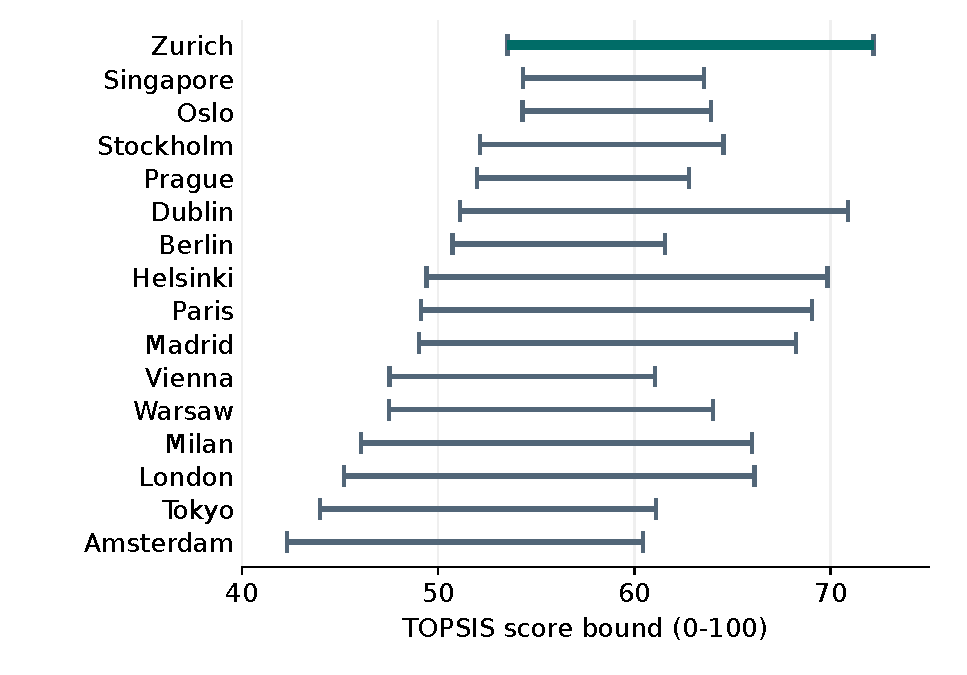
\includegraphics[width=\linewidth]{task4_v154_assets/score_intervals.pdf}
\caption{Current score bounds and conservative decision order for the sixteen
cities. Intervals retain missing information; they are not confidence intervals.
Source: frozen city matrix and admitted supplements.}
\label{fig:intervals}
\end{figure}

\FloatBarrier
\subsection{A significant revision: retaining uncertain evidence}
A controlled comparison shows why evidence bounds belong in the decision.
On the same 160 utility entries, compare the midpoint completion $z_{ij}=(\ell_{ij}+h_{ij})/2$ with the retained-interval formulation in Equation~\ref{eq:regret}. Both use identical weights, anchors and TOPSIS scores. The midpoint is a declared diagnostic scenario, rather than an estimate of missing observations or a reconstruction of the team's historical first model.

The revision retains 48 non-point entries and selects the city with the smallest worst-case shortfall. Zurich remains the recommendation, but 13 cities change decision rank under fixed weights; Kendall's $\tau_b=0.583$. With equal weights, 15 ranks change and $\tau_b=0.650$.

For each target city $c$, construct a separate interior completion: set every uncertain utility to $\ell_{ij}+\alpha_i(h_{ij}-\ell_{ij})$, with $\alpha_c=0.95$ and $\alpha_i=0.05$ for $i\ne c$. All 112 point values remain fixed and all 48 uncertain values lie strictly inside their intervals. Each target ranks first under both baseline and equal weights. Across the sixteen targets, the smallest lead is 4.966 score points under baseline weights and 5.306 under equal weights. These separate completions establish feasibility in the declared utility rectangle; they carry no estimated probabilities and do not establish joint physical attainability.

Retaining intervals changes the decision order while preserving sixteen possible champions. The \TotalWidthReduction\% reduction in interval width comes from admitted data, separately from this formulation comparison.


\subsection{Sensitivity to the accepted input information}\label{sec:sourcepolicy}
The conservative choice depends on which submitted observations are accepted.
Of the 112 retained point entries, 64 are labelled 2026, two 2025 and 46 earlier;
28 carry non-\texttt{ok} source flags: 16 \texttt{MODELLED}, eight \texttt{STALE},
three \texttt{SUSPECT} and one \texttt{NATIONAL}.
For a controlled test, replace selected point utilities by $[0,1]$, keeping
weights, all supplements and the 48 original non-point bounds unchanged.
The groups are points dated before 2020, after 2025, non-\texttt{ok} points and
their union. The union counts overlapping entries once.

\begin{table}[!ht]\centering
\caption{Recommendation after withdrawing selected submitted point information. Width is the mean baseline-weight score range on the 0--100 scale.}\label{tab:vintage}
\begin{tabular}{l r l l r}\toprule
Withdrawn group & Cells & Baseline & Equal & Width\\\midrule
Retained input & 0 & Zurich & Zurich & 16.06 \\
Before 2020 & 13 & Singapore & Zurich & 21.14 \\
After 2025 & 64 & Zurich & Zurich & 48.42 \\
Non-ok flags & 28 & Berlin & Paris & 29.11 \\
Union & 95 & Singapore & Singapore & 68.79 \\
\bottomrule\end{tabular}\end{table}


Withdrawing the 28 flagged points changes the recommendation to Berlin under
baseline weights and Paris under equal weights. Removing the 13 pre-2020 points
selects Singapore under baseline weights; equal weights retain Zurich.
Withdrawing the 64 later-dated points retains Zurich under both references,
while widening the baseline mean range from 16.06 to 48.42. The 95-entry union
selects Singapore under both. All sixteen cities remain possible champions
in every case. These withdrawals test dependence on accepted information:
the labels and date cutoffs are not calibrated error probabilities or a
judgment that every flagged entry is wrong. The experiment preserves the
primary data and does not reconstruct a same-year-only matrix.

Withholding Zurich's homicide-rate point alone selects Singapore under baseline
weights and Oslo under equal weights. Withholding Amsterdam's alone retains
Zurich under both. Each single-point test keeps the other 159 entries fixed;
no official count is inserted as an assumed replacement rate.

Holding the other 159 entries fixed while varying this point rate $x_Z$, Zurich ties Singapore in maximum regret at about $x_Z=0.23002$ per 100,000 under baseline weights, and Oslo at about $x_Z=0.90473$ under equal weights. Below each respective cutoff Zurich uniquely minimizes regret; above it Zurich does not. These are hypothetical point-rate cutoffs, not observed rates or confidence limits.


\section{Model revision and extension}
\subsection{Considering future changes}
We examine three conditional changes while holding anchors and population
denominators fixed. Resource expansion raises higher-education, stop and pool
densities by 10\%. Living pressure raises living costs, housing cost ratios and
travel durations by 10\%. Balanced improvement reduces pupil--teacher ratios,
PM$_{2.5}$ and travel durations by 10\%. A comparable multi-year panel is not
available, so these changes have no estimated annual rate or forecast date.

For raw multiplier $r>0$, the utility transformations are
\begin{equation}
 T_r^{+}(u)=\frac{ru}{1-u+ru},\qquad
 T_r^{-}(u)=\frac{u}{u+r(1-u)}.
\end{equation}
These increasing maps propagate raw-scale changes through benefit and cost
intervals. For known mean travel duration, the new Jensen interval is
$[e^{-r\bar t/30},1]$. Singapore instead has bounds $[L_q,U_q]$ on expected
utility. With $q=e^{-t/30}$ and $t'=rt$, Jensen and $0\leq q\leq1$ give
\begin{equation}
 \mathbb E[q^r]\in
 \begin{cases}
 [L_q,U_q^r],&0<r<1,\\
 [L_q,U_q],&r=1,\\
 [L_q^r,U_q],&r>1.
 \end{cases}
 \label{eq:moment}
\end{equation}
Raising both endpoints to $r$ would generally misrepresent an expected utility.
Equation~\ref{eq:moment} is an outer moment bound and need not be reversible.
Fully missing travel remains unknown. Thus the extension accommodates the
different information supplied by means and by travel distributions.

\FutureDeterministic
We also solve a decision boundary: holding other cities fixed, proportionally
reduce one city's pupil--teacher ratio, PM$_{2.5}$ and travel durations until
its maximum regret ties that of the best other city. \FutureThresholds
These thresholds describe the model response to a specified joint change;
they do not establish policy feasibility or a uniquely identified champion.
\EvidenceThresholdCheck

For a separate future-shock simulation, each draw combines a common shock and
city-specific shocks under a declared bounded distribution, with the criterion
weights held fixed. Original data intervals are not randomly completed.
\FutureMonteCarlo
\ProxyWithdrawalMC
These are conditional stress frequencies under an uncalibrated distribution.
Weight perturbations below answer a separate question and are not blended
silently into the future-shock frequencies.

\subsection{Considering different preferences and development situations}
Education priority doubles the weights of the two education indicators.
The independent living scenario doubles travel and transport-stop weights.
Equation~\ref{eq:weights} then normalizes all weights.
\PreferenceResults
\PreferenceEvidenceChange
The resulting differences show how the definition of a desirable city affects
the decision. They do not establish measured differences between fourteen- and
eighteen-year-old students.

\subsection{Perturbing weights}
For each preference centre $w'$, we draw
$w^{(b)}\sim\operatorname{Dirichlet}(\kappa w')$, with
$\kappa\in\{20,100,500\}$ and 10,000 draws per setting. Every draw recomputes
interval TOPSIS and maximum regret without filling missing values. We report
mean decision rank, fractional first-place recommendation frequency and
fractional top-three decision membership; ties share membership.

\begin{table}[!ht]\centering
\caption{Conditional recommendation frequencies (\%) for selected cities at concentration 100.}
\begin{tabular}{lrrr}\toprule
Preference centre & Zurich & Oslo & Singapore\\\midrule
Baseline & 43.33 & 27.92 & 28.23 \\
Education priority & 6.83 & 42.95 & 41.43 \\
Independent living & 58.99 & 15.46 & 25.12 \\
\bottomrule\end{tabular}\end{table}




\MonteCarloInterpretation
These two summaries optimize different quantities. We retain minimum maximum
regret as the predeclared decision rule; Monte Carlo reports its sensitivity.
Neither average ranks nor a network aggregation resolves the missing empirical
information. A low AHP consistency ratio and repeated simulations demonstrate
calculation properties, not representative student opinion.

\subsection{Within-city fairness and growth stages}
Citywide facilities per resident measure supply. Student access additionally
depends on fees, opening hours, transport, disability access and location;
identifying its distribution requires matched students and qualifying facilities.

\EquityCase
For districts $d$ with pupil counts $n_d$ and pupil--teacher ratios $r_d$,
the pupil-weighted utility is
$\bar u=\sum_d n_d\,15/(15+r_d)/\sum_dn_d$.
Its difference from pooled utility reflects aggregation; school-location data
establish neither resident travel access nor policy effects.

For Istanbul's retained 2012 high-school cohort aged 14--18, let $L_{0.2}$
be the lowest-20\% weighted mean travel utility, with fractional boundary
inclusion, and $\mu$ the overall mean. Unknown utilities lie in $[0,1]$; optional membership remains uncertain. Observed weight is $W=499950$; including all
optional members gives $N_{\max}=681503$. The sharp joint bound is
$\min(\mu-L_{0.2})=(W/N_{\max})(\mu_{\mathrm{obs}}-L_{0.2,\mathrm{obs}})=0.226686$,
where ``obs'' denotes observed trips.
Including all optional members and setting unknown trips to 45 minutes attains it.
With cohort, weights and missing-data rules fixed, allowing arbitrary utility
changes to at most 5\% or 20\% of observed weighted mass leaves sharp minimum gaps
0.200134 or 0.129091, respectively. This fractional-mass relaxation uses declared
error budgets, not estimated error rates or fractions of students.
The official-portal aggregate projection, rather than original CSV bytes,
supports these historical feasibility results, not current facility-use estimates
\cite{istanbul}.

\AgeCase

The shared-membership constraint permits both historical age-group orderings. For younger-minus-older mean travel utility, the joint closure is $[-0.23330,0.26325]$, assigning the shared unknown-age mass once. Two separate completions with unknown utilities 0.05 and 0.95 give contrasts $+0.23842$ and $-0.20848$. Both use finite durations and allocate the shared mass to the younger group. The closure endpoints allow zero utility as a limiting value; the two reversals use strictly interior values. These are feasibility constructions within the retained 2012 aggregate uncertainty set, not observed age effects.


Comparing exact ages fourteen and eighteen requires matched resident utilities
$u_{ij}^{(14)},u_{ij}^{(18)}$ and separately elicited weights
$w_j^{(14)},w_j^{(18)}$. Our analyst preference scenarios carry no age labels.

\section{Comparing cities within the same country}
Every primary city belongs to a different country, so the main sample cannot
identify within-country city contrasts. We use the existing United States and
India cases as frozen legacy25 V117 examples with the same ten indicator
definitions and scoring formula \cite{legacycase}. They do not enter the sixteen-city ranking,
and comparison within a country does not remove differences in source year,
city boundary or educational coverage.

\begin{table}[!ht]\centering
\caption{Separate historical country cases using the legacy 25-city V117 evidence.}
\begin{tabular}{llr}\toprule
Country & City & Score interval\\\midrule
United States & Phoenix & 31.39--71.68 \\
 & New York & 30.22--72.81 \\
India & Mumbai & 28.82--60.64 \\
 & Delhi & 32.59--63.90 \\
\bottomrule\end{tabular}\end{table}


\CountryInterpretation
Affordability contrasts use Numbeo's 2025 named-city aggregates
\cite{numbeocase}; the Mumbai--Delhi air contrast uses 2021 WHO monitoring
means \cite{whocase}. These source scopes are retained in the case source index.
These descriptive contrasts do not identify a national causal effect.

\section{Conclusion and decision use}
Zurich minimizes maximum regret under baseline and equal weights; all sixteen
cities remain possible champions. Education priority selects Oslo. Withholding
Zurich's unverified homicide point selects Singapore under baseline and Oslo
under equal weights; broader withdrawal of 28 flagged points selects Berlin and
Paris, respectively. Families should examine both their priorities and the
source bounds behind a recommendation.

Verified supplements reduce mean score-interval width by 14.62\% while preserving
submitted values. Holding this evidence fixed, the interval revision changes
13 decision ranks and retains completions in which another city outranks Zurich.
Better evidence narrows uncertainty; the decision rule makes that uncertainty
explicit.

\clearpage
\phantomsection\addcontentsline{toc}{section}{News article}\label{news-start}
\section*{A city choice built around a student's day}

Under the retained team inputs, Zurich is the cautious recommendation emerging from our comparison of sixteen cities for high-school life. An alternative that places greater emphasis on education points to Oslo. Together, these findings offer students and families a practical starting point: a city comparison that connects everyday opportunities with personal priorities while keeping gaps in the evidence visible.

For a teenager, choosing a city involves the school day and the hours around it. Teaching resources, nearby higher education, clean air, safety, housing and living costs, transport, journey times, internet access and swimming facilities can all matter. Our study brings these ten considerations into one framework. Its purpose is to help families examine trade-offs, rather than assume that the same place will suit every student.

\subsection*{A cautious recommendation with a clear meaning}

The comparison uses common scoring yardsticks and a stated balance of priorities. Where a figure is missing or describes part of a city's resources, the model keeps a range of possible scores. An unknown figure therefore remains open rather than being replaced with an invented average. Each city's overall result is a range, reflecting the information available under the model's assumptions.

The recommendation asks how far a selected city could fall behind a better-scoring alternative within those ranges. Zurich has the smallest worst-case shortfall under the baseline priorities. It also remains the cautious recommendation when all ten considerations receive equal weight. This makes it a useful place to begin a broad comparison; all sixteen cities nevertheless remain possible leaders within the retained evidence ranges. The study has not established a single certain winner.

\subsection*{Better evidence makes the comparison more useful}

Official records become useful when their boundaries and units are clear. Vienna's broad transport register contains depot objects whose status as passenger stops is unproved. Cross-checking the operator list with a separate city map confirms 99 metro station areas. Prague's city list supplies 57 metro complexes after interchanges are counted once and a closed station is omitted. These examples show why a useful inventory needs more than a headline total.

Across twenty-two previously missing entries, additional evidence reduced the average width of the city score ranges by about 15 per cent. The original submitted values and scoring rules stayed in place. Narrower ranges make the comparison more informative, while the full set of possible leaders shows that further evidence could still change the conclusion. The records span different years, and some describe school or city resources rather than the experience of a particular teenager.

\newpage
\subsection*{Students' priorities can change the recommendation}

In an education-focused comparison, the relative emphasis on teaching resources and the density of higher-education institutions is doubled before the priorities are balanced again. Oslo then becomes the cautious recommendation. This is an illustrative choice made by the analysts, not a finding from a student survey. It gives a family a concrete way to explore how a stronger educational emphasis changes its shortlist.

City totals also need a local check. A transport-stop inventory leaves questions about walking distance, service frequency, fares and accessible routes. A pool count leaves questions about entry fees, opening hours and which neighbourhoods the facilities serve. These are useful questions for families and city planners to investigate before treating resource supply as equal access. The study does not measure an individual student's benefit from adding a stop, teacher or pool.

\subsection*{Use future scenarios to ask better questions}

The study also examines three hypothetical changes: expanding selected resources, increasing living and travel pressures, and reducing selected educational, air-quality and travel burdens. When the affected quantities change uniformly by ten per cent, Zurich remains the cautious recommendation under both baseline and equal priorities. Repeated simulations explore what happens when the assumed changes differ across cities. They test chosen scenarios; they do not predict a future year or estimate a city's real chance of being best.

Checking a specific source can change the shortlist: treating Zurich's unverified homicide-rate figure as unknown points to Singapore under the original priorities and Oslo with equal priorities. The original figure remains in the declared baseline; no replacement rate is assumed.

A family's next step is to pair the city comparison with its own school options, budget, daily route and preferred activities. Students can give education more emphasis, examine the affordability trade-offs, and check whether nearby opportunities fit their routines. The model makes those choices easier to discuss: a clear starting recommendation, room for different priorities, and an explicit view of the evidence needed for a more personal decision.
\label{news-end}
\clearpage
\phantomsection\addcontentsline{toc}{section}{References}
% Owned references rebased to V154 evidence and controlled analyses.
\begin{thebibliography}{99}
\raggedright
\bibitem{teamtable} Team-supplied city-indicator table, sixteen cities.
Frozen input archived November 2026; original values, years and flags retained.
\bibitem{saaty} T. L. Saaty. The analytic hierarchy process---what it is and
how it is used. \textit{Mathematical Modelling}, 9(3--5), 161--176, 1987.
\url{https://doi.org/10.1016/0270-0255(87)90473-8}.
\bibitem{topsis} C.-L. Hwang and K. Yoon. \textit{Multiple Attribute Decision
Making: Methods and Applications}. Springer, 1981.
\url{https://doi.org/10.1007/978-3-642-48318-9}.
\bibitem{vikor} S. Opricovic and G.-H. Tzeng. Compromise solution by MCDM
methods: A comparative analysis of VIKOR and TOPSIS.
\textit{European Journal of Operational Research}, 156(2), 445--455, 2004.
\url{https://doi.org/10.1016/S0377-2217(03)00020-1}.
\bibitem{oslo} City of Oslo, municipal transport GIS, layer 800; Norwegian
Mapping Authority, municipality 0301 boundary. Accessed November 2026.
\url{https://geodata.bymoslo.no/arcgis/rest/services/geodata/Temadata_Publikum/MapServer/800}.
\bibitem{vbz} Verkehrsbetriebe Z\"urich. \textit{Zahlen und Fakten 2025}, p.~6.
\url{https://www.stadt-zuerich.ch/content/dam/vbz/de/die-vbz/zahlen-fakten/geschaeftsbericht/Z4690_VBZ_FB-2025_Web.pdf}.
\bibitem{helsinki} Metropolitan Area Transport Ltd. \textit{Metrolla}.
Official operator inventory, accessed November 2026.
\url{https://kaupunkiliikenne.fi/liikennointi/metrolla/}.
\bibitem{stockpool} City of Stockholm. \textit{Simhallarna} and current swimming
overview. Accessed 8 November 2026.
\url{https://motionera.stockholm/trana-gymma-simma/simhallarna/}.
\bibitem{apur} Atelier parisien d'urbanisme. \textit{Atlas des activit\'es \`a
Paris}, March 2022, p.~37. Sources RATP 2021 and Apur 2022.
\url{https://www.apur.org/sites/default/files/atlas_activites_paris_immobilier.pdf}.
\bibitem{prague} Czech Statistical Office. \textit{Schools and school facilities,
2024/25}, Tables 3.1.3 and 6.1.18.
\url{https://csu.gov.cz/docs/107508/299702e7-bc0a-1dc2-87db-600d0303f2f4/23004225.pdf?version=1.1}.
\bibitem{kolada} RKA/Kolada, indicator N17816, Stockholm municipality 0180,
period 2025; source Skolverket (Siris). Definition and total-provider scope
archived with the API response.
\url{https://api.kolada.se/v3/data/kpi/N17816/municipality/0180/year/2025}.
\bibitem{parisedu} Acad\'emie de Paris. \textit{Chiffres cl\'es 2025},
2024 school-entry pupils and 31 December 2024 teacher totals.
\url{https://www.ac-paris.fr/sites/ac_paris/files/2025-08/chiffres-cl-s-acad-mie-de-paris-44994.pdf}.
\bibitem{singapore} Singapore Department of Statistics. \textit{Census of
Population 2020, Statistical Release 2}, Tables 93 and 124; official Parliament
mirror and official data API.
\url{https://www.parliament.gov.sg/docs/default-source/default-document-library/cop2020sr2.pdf}.
\bibitem{dublin} Dublin City Council and National Transport Authority.
\textit{Dublin City Centre Transport Plan 2023, Technical Note 6},
issued 2024, Figure 3-7.
\url{https://www.dublincity.ie/sites/default/files/2024-04/06-dublin-city-centre-transport-plan-public-transport-technical-note.pdf}.
\CaseReferences
\bibitem{openai} OpenAI. Codex, AI-assisted research, coding, checking and writing
environment. Used 8--9 November 2026; recorded client
\texttt{0.166.0-alpha.5.1}, task model identifier \texttt{gpt-6.1-sol}.
Immutable serving build and complete team history not established.
\url{https://openai.com/codex/}.
\bibitem{exa} Exa. \texttt{web\_fetch\_exa}, official-source retrieval and text
extraction. Used 8--9 November 2026; internal model and service version not
recorded in saved receipts. \url{https://exa.ai/}.
\bibitem{legacycase} Study archive. Frozen legacy25 V117 utility intervals:
Phoenix--New York and Mumbai--Delhi case subsets, November 2026. Retained
separately from the primary sixteen-city evidence; source index and selected
case utilities accompany this review draft.
\bibitem{numbeocase} Numbeo. \textit{Quality of Life Index by City 2025},
cost-of-living index excluding rent and property price-to-income ratio.
Named-city crowdsourced aggregates; administrative boundaries not
independently harmonized.
\url{https://www.numbeo.com/quality-of-life/rankings.jsp?title=2025}.
\bibitem{whocase} World Health Organization. \textit{Ambient Air Quality Database},
June 2026 update. Mumbai and Delhi PM$_{2.5}$ monitoring means refer to 2021;
two stations and one station respectively, with temporal coverage unreported.
\url{https://www.who.int/publications/m/item/who-ambient-air-quality-database-(update-jun-2026)}.
\bibitem{madridmetro} Consorcio Regional de Transportes de Madrid. M4 Estaciones, register dated 29 May 2026; municipality code and network-station identifiers. Accessed 9 November 2026.
\url{https://services5.arcgis.com/UxADft6QPcvFyDU1/arcgis/rest/services/M4_Red/FeatureServer/0}.
\bibitem{inecodes} Instituto Nacional de Estad\'istica. Transport statistics metadata, municipal classification, 2026.
\url{https://www.ine.es/dynt3/metadatos/RespuestaDatos.html?oper=297}.
\bibitem{nerimapool} Nerima City. Municipal swimming inventory and linked venue pages, accessed 9 November 2026.
\url{https://www.city.nerima.tokyo.jp/shisetsu/koen/index.html}.
\bibitem{nerimaclose} Nerima City. Heiwadai closure, 27 October 2026; Miharadai planned closure, 29 September 2026.
\url{https://www.city.nerima.tokyo.jp/kankomoyoshi/sports/oshirase/20261027.html};
\url{https://www.city.nerima.tokyo.jp/kankomoyoshi/sports/oshirase/20260929.html}.
\bibitem{irelandfte} Department of Education and Youth, Ireland. \textit{Teacher Workforce Data Quality Report}, 2026, Sections 5.2 and 8.4.
\url{https://nationaldata.ie/media/NationalDataie/MethodologyDocumentation/Teacher_Workforce_Data_Quality_Report.pdf}.
\bibitem{viennaogd} Wiener Linien. Versioned operator OGD files and
\textit{Beschreibung der OGD-Dateien}, v1.3 (2022), p.~4. Export version
8 November 2026; accessed 9 November 2026. DIVA station areas are distinguished
from individual stopping positions.
\url{https://www.wienerlinien.at/ogd_realtime/doku/}.
\bibitem{viennagis} City of Vienna. Existing U-Bahn stops and Vienna boundary,
OGD WFS layers \texttt{UBAHNHALTOGD} and \texttt{LANDESGRENZEOGD}.
Accessed 9 November 2026; boundary record dated 1 September 2026.
Datenquelle: Stadt Wien -- data.wien.gv.at.
\url{https://data.wien.gv.at/daten/geo?service=WFS&request=GetCapabilities}.
\bibitem{pidmetro} Prague Integrated Transport (PID). \textit{Zast\'avky v Praze},
Prague-only station lists and linked metro timetables, accessed 9 November 2026.
\url{https://pid.cz/zastavky-pid/zastavky-v-praze/}.
\bibitem{dpp2025} Dopravn\'i podnik hlavn\'iho m\v{e}sta Prahy.
\textit{Annual Report 2025}, PDF pp.~17 and 103. Line appearances and
distinct interchange complexes retained separately.
\url{https://www.dpp.cz/spolecnost/o-spolecnosti/vyrocni-zpravy}.
\bibitem{floraclose} Dopravn\'i podnik hlavn\'iho m\v{e}sta Prahy.
Flora station closure from 2 February 2026 until further notice; Florenc C
partial accessibility restriction. Accessed 9 November 2026.
\url{https://www.dpp.cz/omezeni-a-mimoradne-udalosti/detail/15};
\url{https://www.dpp.cz/omezeni-a-mimoradne-udalosti/detail/39}.
\bibitem{bvg} Berliner Verkehrsbetriebe (BVG). U1--U9 official route profiles and tariff-zone definitions. Native station identifiers, station-level zone A and interchange declarations; accessed 9 November 2026.
\url{https://www.bvg.de/de/verbindungen/linienuebersicht}
\url{https://www.bvg.de/de/abos-und-tickets/tarifzonen-und-tarifbestimmungen}
\bibitem{deppmatch} Minist\`ere de l'\'Education nationale, DEPP. Institution personnel indicators and general/technological lyc\'ee pupil counts, rentr\'ee 2025; Henri-IV UAI 0750654D. Teacher ETP covers the institution, not a published upper-stage allocation. Accessed 9 November 2026.
\url{https://data.education.gouv.fr/explore/dataset/fr-en-indicateurs_personnels_etablissements2d/}
\url{https://data.education.gouv.fr/explore/dataset/fr-en-lycee_gt-effectifs-niveau-sexe-lv/}
\bibitem{deppdirectory} Minist\`ere de l'\'Education nationale. Official school directory, Henri-IV UAI 0750654D, row updated 7 November 2026; post-baccalaureate flag. Accessed 9 November 2026.
\url{https://data.education.gouv.fr/explore/dataset/fr-en-annuaire-education/}
\bibitem{tflinventory} Transport for London. Unified API, tube-mode StopPoint inventory and StopTypes metadata; accessed 9 November 2026. Native station and hub identifiers distinguish station entities from platforms and entrances.
\url{https://api.tfl.gov.uk/StopPoint/Mode/tube}
\url{https://api.tfl.gov.uk/StopPoint/Meta/StopTypes}
\bibitem{onslondon} Office for National Statistics. Regions (December 2025) Boundaries EN BFC, full-resolution coastline-clipped geometry; London region E12000007. Accessed 9 November 2026.
\url{https://services1.arcgis.com/ESMARspQHYMw9BZ9/arcgis/rest/services/Regions_December_2025_Boundaries_EN_BFC/FeatureServer/0}
\bibitem{warsaw2022} PBS/TRAKO for the Warsaw Metropolitan Area. \textit{Raport nr 2 z diagnozy zachowa\'n transportowych mieszka\'nc\'ow}, July 2022, pp.~3--4, 58, 64. Fieldwork 12 March--30 April 2022; city school-travel sample base 22. Original retrieved 9 November 2026.
\url{https://omw.um.warszawa.pl/wp-content/uploads/2022/09/Raport-nr-2-glowny.pdf}
\bibitem{cbshomicide2022} Statistics Netherlands (CBS). \textit{Meer mensen vermoord in 2022, meeste slachtoffers in Rotterdam}, 29 August 2023; provisional annual city table, and accompanying \textit{Slachtoffers moord en doodslag 2022}, Table 7, period 2018--2022. Originals retrieved 9 November 2026.
\url{https://www.cbs.nl/item?sc_itemid=209e5ed2-506c-42d6-b414-49d3556810bf}
\url{https://www.cbs.nl/nl-nl/maatwerk/2023/35/slachtoffers-moord-en-doodslag-2022}
\bibitem{zhpks2025} Kantonspolizei Z\"urich. \textit{Polizeiliche Kriminalstatistik Kanton Z\"urich 2025}, pp.~117--118, city totals and definition of a criminal act. Original retrieved 9 November 2026.
\url{https://www.zh.ch/content/dam/zhweb/bilder-dokumente/themen/sicherheit-justiz/delikte-praevention/dokumente/pks/aktuell/jahresbericht_2025.pdf}
\bibitem{sgbus_lta} Land Transport Authority, Singapore. Bus Stop Location,
Data.gov.sg catalogue and GeoJSON; retrieved 7 November 2026. Archived original
geometry and catalogue HTML; count uses distinct nonempty native bus-stop codes.
\url{https://data.gov.sg/datasets/d_3f172c6feb3f4f92a2f47d93eed2908a/view}
\bibitem{sgpool_2025} Sport Singapore, ActiveSG Circle. \textit{Editors' pick:
must-hit pools in Singapore}, published 23 April 2025; retrieved 8 November
2026. Archived provider-extracted text and linked venue details; current
pages corroborate venue identity, not 2025 opening hours.
\url{https://www.activesgcircle.gov.sg/read/editors-pick-must-hit-pools-in-singapore}
\bibitem{warsawedu2025} Statistical Office in Warszawa. \textit{Statistical
Yearbook of Warsaw 2025}, education workbook and PDF pp.~156--160, 165;
rounding note p.~22. School-year 2024/25 tables; archived original workbook.
\url{https://new.stat.gov.pl/en/publications-portal/statistical-yearbook-warsaw-2025}
\bibitem{zurichpool} City of Z\"urich. Municipal indoor swimming-pool directory,
retrieved 8 November 2026; archived provider-extracted representation.
Current directory snapshot, including W\"armebad K\"aferberg.
\url{https://www.stadt-zuerich.ch/de/stadtleben/sport-und-erholung/sport-und-badeanlagen/hallenbaeder.html}
\bibitem{milanpool2025} Milanosport. Swimming-pool tariffs effective 1 June
2025, updated 9 October 2025. Retrieved 8 November 2026; archived
provider-extracted PDF representation, tariff groups A and B.
\url{https://www.milanosport.it/workspace/uploads/nuovi-tariffari-1-giugno-2025-agg-9-10-2025.pdf}
\bibitem{stockholmmetro2025} City of Stockholm and Local Police Area
V\"allingby. \textit{L\"agesbild 2025}, PDF p.~11 (printed p.~10),
Bromma and H\"asselby-V\"allingby metro stations; retrieved 8 November 2026.
Archived original report.
\begingroup\def\UrlBreaks{\do\/\do-\do\?}\url{https://meetingspublic.stockholm.se/welcome-sv/namnder-styrelser/hasselby-vallingby-stadsdelsnamnd/mote-2025-12-18/agenda/6-lagesbild-2025-samverkansoverenskommelse-mellan-hasselby-vallingby-sdf-och-lokalpolisomrade-vallingbypdf?downloadMode=open}\endgroup
\bibitem{milanmetro} Comune di Milano. Stazioni\_Metro, ATM\_Metro MapServer layer 0; metadata date 16 October 2024. Original station and ID responses retrieved November 2026; municipal code 015146 and five operator-map interchange pairs retained.
\url{https://gisportal.comune.milano.it/server/rest/services/D_Mobilita/ATM_Metro/MapServer/0}.
ATM, metro/suburban network map, V26B label, publication date unreported.
\url{https://www.atm.it/it/AltriServizi/Trasporto/Documents/schema_rete_metro.pdf}.
\bibitem{irelandpayroll} Department of Education and Youth.
\textit{The Teaching Workforce in Ireland: Primary and Post Primary Level,
2025/26 School Year}. April 2026, Table 10, p.~14; November 2025 payroll.
\url{https://assets.gov.ie/static/documents/5935f213/Teacher_Workforce_Data_Report_2026.pdf}.
\bibitem{finlandfte} Statistics Finland / Eurostat. Finland UOE national
reference metadata, Annex III--Additional tables, sheet 15.2.2, cell F10.
National metadata updated 1 October 2026; original workbook retrieved
9 November 2026. Full-time/part-time and FTE estimation methods.
\url{https://ec.europa.eu/eurostat/cache/metadata/Annexes/educ_uoe_enr_esmsed_fi_an_Annex_III_-_Additional_tables.xlsx}.
\end{thebibliography}
\label{main-end}
\clearpage
\section*{Report on Use of AI Tools}
\addcontentsline{toc}{section}{Report on Use of AI Tools (additional pages)}
\textbf{Documentation status: incomplete review record.}
This appendix records assistance supported by saved task metadata and research
receipts. The complete team AI history remains to be reconciled with actual
saved conversations and other tool records before submission.

\subsection*{Known tool and scope}
\textbf{OpenAI Codex}, used 8--9 November 2026. The task log records Codex
Desktop client version \texttt{0.166.0-alpha.5.1} and model identifier
\texttt{gpt-6.1-sol} in all 28 saved turn contexts within the inspected prefix.
The identifier does not expose an immutable serving build or establish the
model used by every concurrent assistant. The assistant supported official-source
search and extraction, data-scope checks, Python calculations and audits,
LaTeX drafting, and wording revisions. Concurrent assistant tasks prepared
bounded evidence checks, a controlled model diagnostic and the news-article
contribution \cite{openai}. The anti-defensive-writing skill supplied editorial instructions;
it is a workflow resource, not a surveyed student preference or a data source.

\textbf{Exa}, used 8--9 November 2026 through the recorded
\texttt{web\_fetch\_exa} tool, retrieved and extracted text from official
webpages, PDFs and data interfaces \cite{exa}. Saved receipts identify the
service, source URLs and returned text, but do not specify an internal model
or service version. They do not establish whether a generative model
participated in every extraction. Extracted representations are distinguished
from original downloaded bytes. For example, Tokyo sports-facility PDF text
with ambiguous row order was excluded; the admitted five-venue lower bound
uses separately downloaded Nerima municipal HTML.

\clearpage
\subsection*{Recovered records and coverage}
A complete-line prefix of the local task log is authenticated by its byte count
and SHA-256 in the supporting metadata inventory. That prefix ends at
03:17 UTC on 9 November 2026; later continuations are outside its coverage.
A private export preserves
four genuine request messages, 99 visible progress messages and 22 complete
visible final messages, with per-record hashes. It excludes reasoning, internal
instructions, injected continuations and tool payloads. Consequently it does
not cover generated code or manuscript text contained in tool calls, earlier
tasks, attachments or other team members' use. The raw local log and private
export are not included as submission transcripts. No missing prompt or output
has been reconstructed and labelled as an exact historical quotation.

\subsection*{Verification associated with this draft}
The research calculations preserve the original city CSV and the V154 primary
evidence. The V154 validation independently recomputes weighted norms and
self-excluded competitor maxima, verifies interval membership of constructed
completions and checks source hashes. Original provider records are kept
separately from derived tables. Compilation and rendered-page review check the
presentation. These checks establish the specified calculation and document
properties; they do not replace the team's responsibility to review factual
claims, original supplied data and final authorship.

\subsection*{Records required to finalize this report}
The final report must identify every AI tool actually used, its available
model or version, date and purpose, and associate relevant use with the text
and references. Actual saved query and response records should be inserted
according to the applicable COMAP policy, including its stated exceptions.
Other team members' tools, translation use and earlier conversations remain
to be confirmed from their records.

The current in-text disclosure and references identify Codex and Exa
assistance. Submission readiness also requires a verified Team Control Number
in place of the review header and confirmation that this report accounts for
the team's actual use.

\end{document}
